\section{Server} \label{sec:Server}
\subsection{Scanner} \label{subsec:Scanner}
Der Scanner wird benötigt, um alle beteiligten Game Clients zu überwachen. Überwacht werden die angebotenen Service auf deren Erreichbarkeit und Absicherung. Die Ergebnisse werden abgesichert, um so die Service Punkte der Gruppen zu berechnen. Auch werden die Ergebnisse für die Dokumentation gespeichert.

\begin{center}
	\includegraphics[width=\linewidth]{entwurf/class_scanner}
	\captionof{figure}{Klassen des Scanners (Klassendiagramm)}
\end{center}

Der Scanner besteht aus der Klasse Scanner, der abstrakten Klasse Scan Operation sowie den abgeleiteten Scan Operationen. Die Klasse Scan Opertion definiert die abstrakte Funktion start(). Diese Funktion wird von den abgeleiteten Klassen implementiert und ermöglicht das starten der einzelnen Scan Operationen. Ebenfalls speichern alle Scan Operationen ihr Ergebnis in der privaten Variable result. Mithilfe der von der abstrakten Klasse implementierten Funktion get\_results() kann der Scanner die Ergebnisse der Scan Operation auslesen. Jeder Scanner startet 0 bis n Scan Operationen abhängig von seiner Konfiguration / den aktiven Diensten. Des Weiteren stellt die abstrakte Klasse die Funktion is\_port\_open bereit, welche von den meisten Scan Operationen genutzt wird. Ein Scanner kann max. pro Typ eine Scan Operation starten und beinhaltet / verwaltet alle Scan Operationen für ein Game Client. Um mehrere Game Clients zu überwachen, werden mehrere Objekte der Klasse Scanner benötigt.

\includegraphics[width=\linewidth]{entwurf/state_scanner}
\captionof{figure}{Ansicht des Scanners (Zustandsdiagramm)}

Bei Starten des Scanners wird die zu bearbeitende Aufgabe spezifiziert.

Sollte der Scanner die Aufgabe \textquote{INIT} bekommen, soll der Scanner die Service Datenbank mit den implementieren Scannern inkl. der Namen füllen, sodass Administratoren diese an- oder ausschalten können.
Um die Service Datenbank zufüllen wird zunächst ein Dummy der Klasse Scanner angelegt. Aus diesem Dummy Objekt werden von allen Scann-Operationen die Namen ausgelesen. Nach dem Auslesen alle Operationen werden die erhalten Daten gebündelt in die Service Datenbank geschrieben und das Programm beendet sich.

Falls die Aufgabe des Scanners \textquote{SCAN} ist, wird der Scann der Game Clients gestartet. Hierzu werden die teilnehmenden Gruppen und der Scanner Timeout aus der Datenbank ausgelesen. Neben diesem werden die aktiven Scanner aus der Datenbank abgefragt. Sind all diese Informationen vorhanden, wird für jede Gruppe ein Scanner erstellt. Bei der Erstellung werden die aktiven Scann-Operationen sowie die Gruppe übergeben. Der Scanner legt dann die benötigten Scann-Operationen an.

\begin{center}
\includegraphics{entwurf/state_scanner_create}
\captionof{figure}{Erstellung eines Scanners (Zustandsdiagramm)}
\end{center}

Nach dem Anlegen der Scanner werden diese nebenläufig gestartet und es wird auf das Beenden der verschieden Scanner gewartet. Sollten alle Scanner mit der Scannrunde fertig sein, wird geprüft, ob das Durchführen einer Scannrunde an den REST-Server gemeldet werden soll. Ist dieses der Fall, wird der Server in Kenntnis gesetzt, dass neue Daten in der Datenbank vorhanden sind. Nachdem diese Aufgaben abgehandelt worden sind, schläft der Scanner bis zu seinem nächsten Durchlauf.

\begin{minipage}{\linewidth}
	\begin{center}
		\includegraphics[height=\textheight]{entwurf/state_scanner_start}
		\captionof{figure}{Starten eines Scanners (Zustandsdiagramm)}
	\end{center}
\end{minipage}

Beim Starten des Scanners wird zu nächst geprüft, ob das entfernte System erreichbar ist. Sollte dieses nicht der Fall sein, werden alle nachfolgenden Scann-Operationen nicht durchgeführt, da diese fehlschlagen werden. Im Anschluss wird getestet, ob der HTTP Dienst des entfernten Systems erreichbar ist, da dieser für einige weitere Tests benötigt wird. Ist der HTTP Dienst erreichbar werden, die Scann-Operationen, welche auf dem HTTP Dienst basieren, mit in die Liste der abzuarbeiten Scann-Operationen aufgenommen. Danach werden alle verbleibenden Scann-Operationen nebenläufig gestartet. Nachdem die Scann-Operationen ihre Aufgabe abgeschlossen haben, sammelt der Scanner alle Ergebnisse ein. Falls die Host UP Scann-Operation oder die HTTP UP Scann-Operation deaktiviert ist, werden diese aus dem Ergebnisse entfernt. Danach übermittelt der Scanner die Daten zur Datenbank und beendet seine Scannrunde.

\paragraph{Scann-Operationen}

Die Scann-Operationen werden nebenläufig abgearbeitet, um so die Dauer eines kompletten Scans zu minimieren. Eine Scann-Operation prüft genau einen Dienst / eine Schwachstelle auf dem entfernten Rechner. Die im alten System implementieren Scans werden in die Scann-Operationen überführt. Deshalb sollen die folgenden Scann-Operationen implementiert werden.

\begin{itemize}
	\item Host-Up
	\item Bubble-Up
	\item BubbleNg-Up
	\item FTP-Save
	\item Htaccess-Save
	\item SQL-Injection-Save
	\item SQL-Password-Save
	\item Telnet-Save
	\item HTTP-UP
	\item HTTPS-UP
	\item XSS-Save
\end{itemize}

\begin{center}
	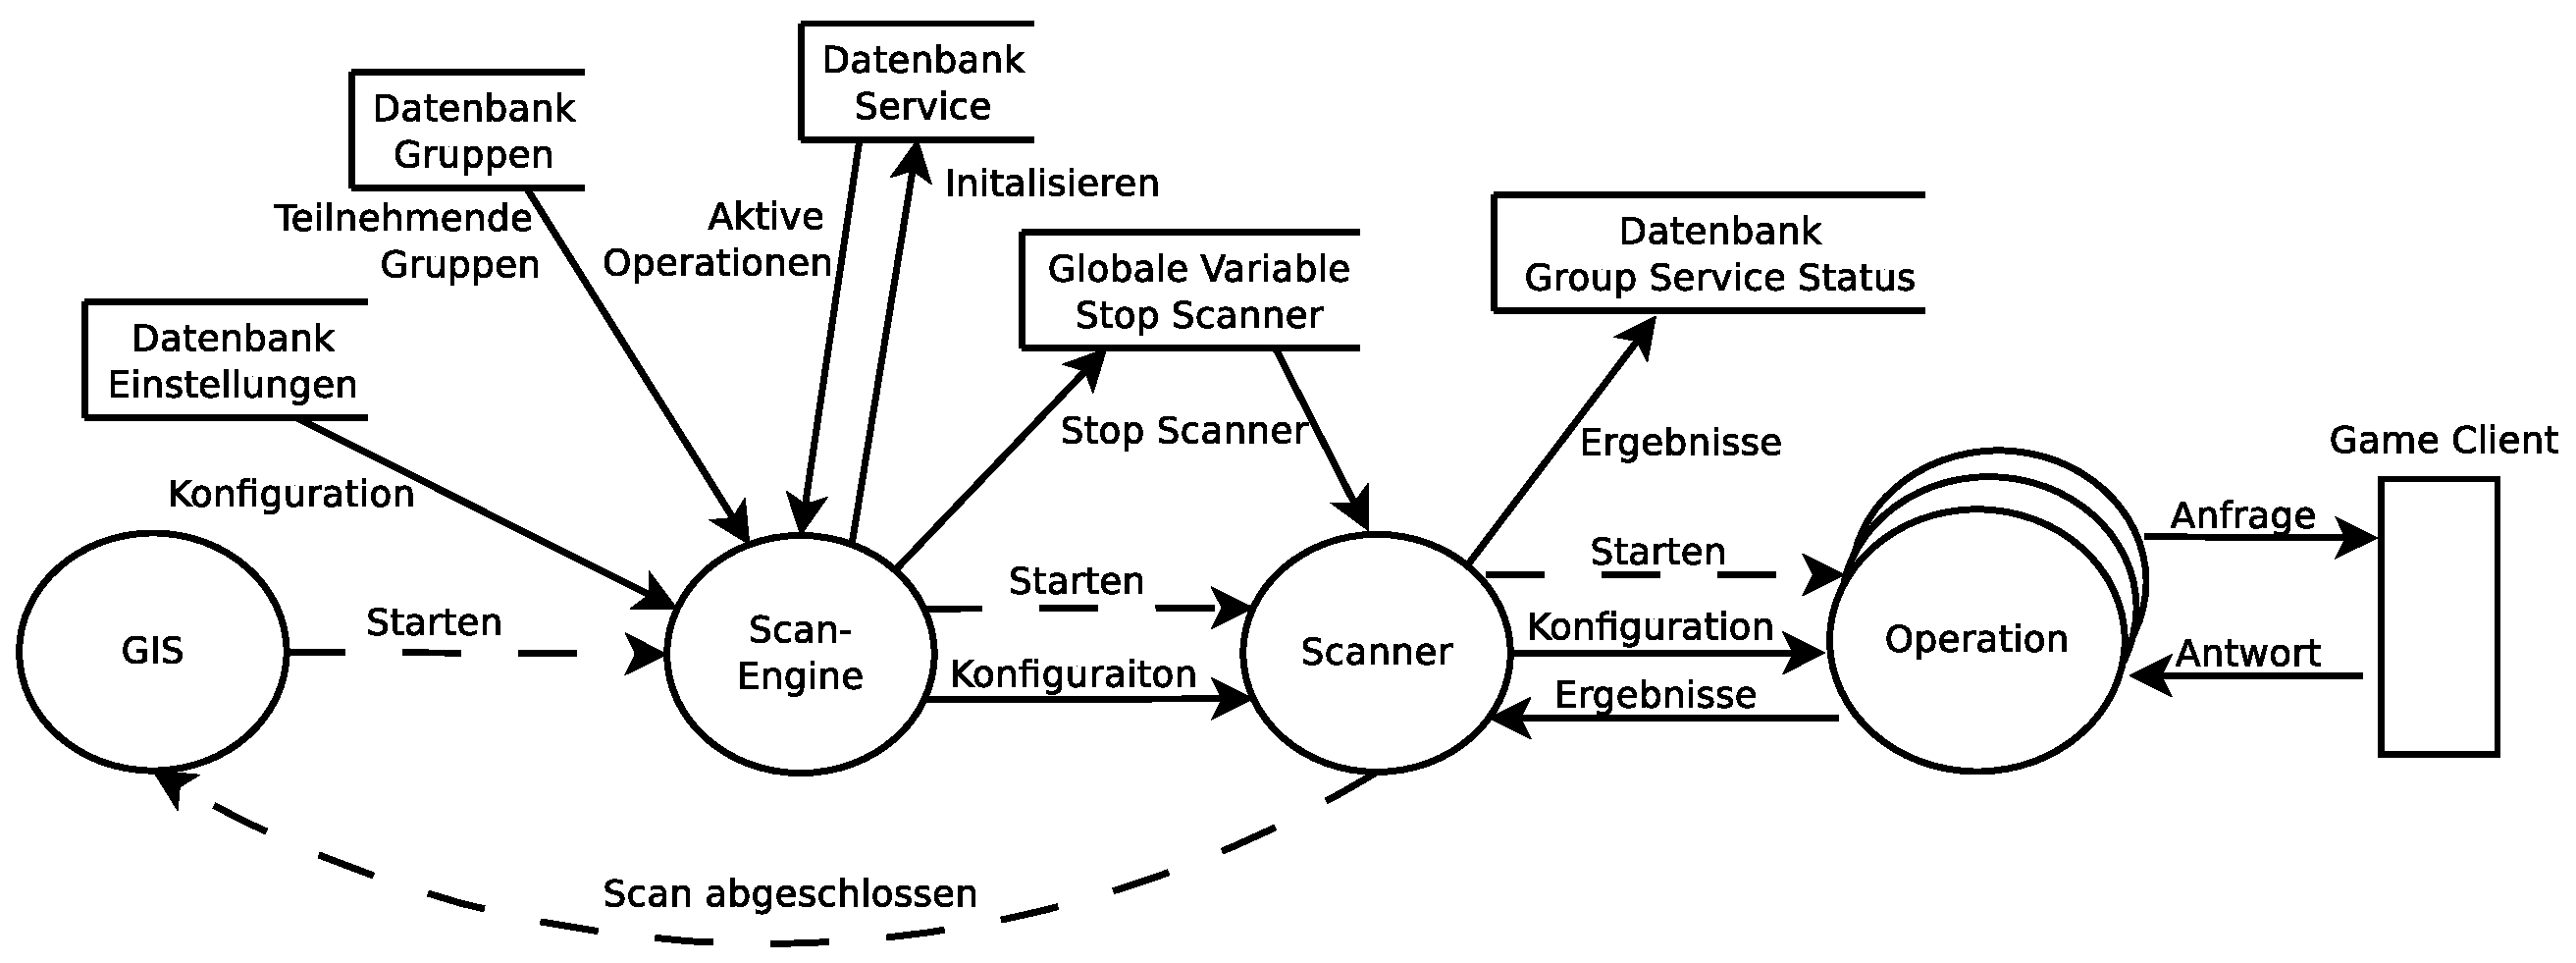
\includegraphics[width=\linewidth]{entwurf/dfd-scanner}
	\captionof{figure}{Datenfluss in der Scanner Komponente (Datenflussdiagramm)}
\end{center}

Die bisher nicht beschrieben Datenflüsse finden zwischen Watchdog und dem Scanner oder zwischen einer Scann-Operation und dem Game Client statt. Administratoren können über Watchdog den Scanner an- bzw. abschalten. Die Scann-Operationen frag bei dem Game Client ihren überwachten Dienst / ihre überwachte Schwachstelle an und erhalten eine Antwort zurück. Anhand dieser Antwort bestimmten die Scann-Operationen das Ergebnis.

\subsection{REST-Interface} \label{subsec:REST-Interface}